% 2015 | UIBK
% vim:set spell tw=79:

\documentclass[beamer]{uibk}
\title{SLIP}
\subtitle{Serial Line Internet Protocol}
\author{Artur Fedrigolli, Roland Gritzer, Martin Pfeifhofer }
\date{\today}

%\AtBeginSection[] {
%\begin{frame}{Outline}
%\tableofcontents[currentsection]
    %\end{frame}
%}
\hypersetup{
    colorlinks,
    citecolor=black,
    filecolor=black,
    linkcolor=black,
    urlcolor=black
}
\graphicspath{ {./media/} }


\begin{document}

\maketitle

\begin{frame}{Problem}
  Wir schreiben das Jahr 1988.

  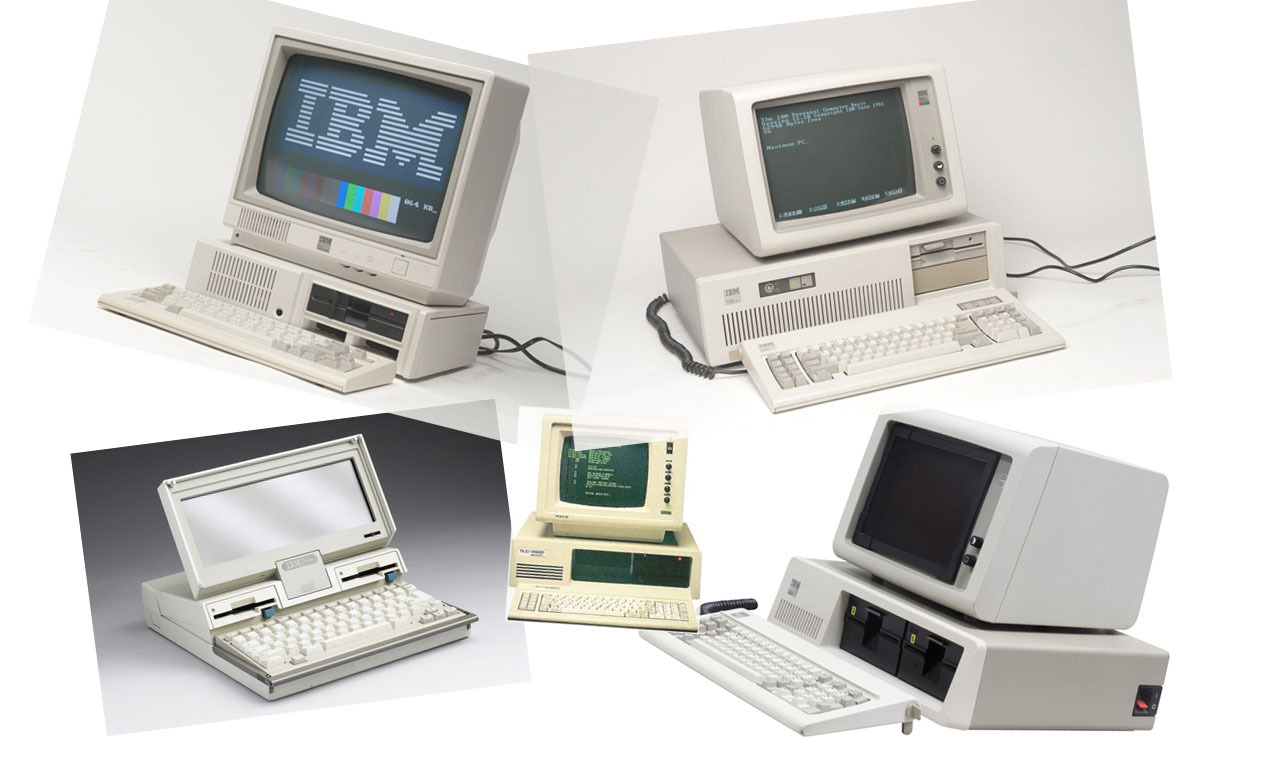
\includegraphics[scale=0.5]{1988computer.jpg}

\end{frame}

\begin{frame}{Ansatz}
  IP Pakete über die serielle Schnittstelle  übertragen
  \begin{center}
  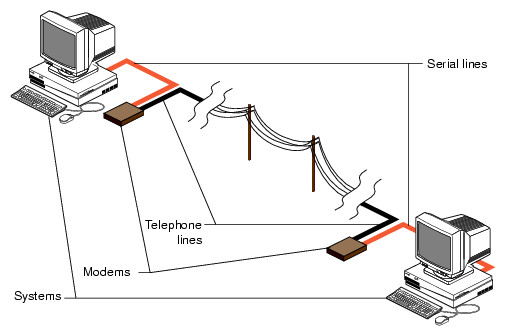
\includegraphics[scale=0.5]{ansatz.jpg}
  \end{center}
\end{frame}

\begin{frame}{Einordnung}

  \begin{center}
  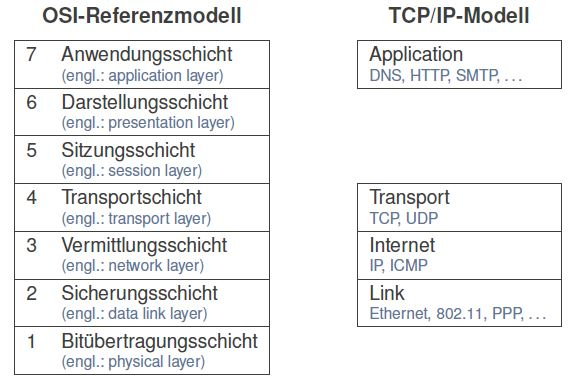
\includegraphics[scale=0.5]{layer.jpg}
  \end{center}

\end{frame}

\begin{frame}{Details}
  \newpage
  \begin{center}
  
\includegraphics[scale=0.5]{ip1.png}
  \end{center}

\end{frame}

\begin{frame}{Details}
  \newpage
  \begin{center}
  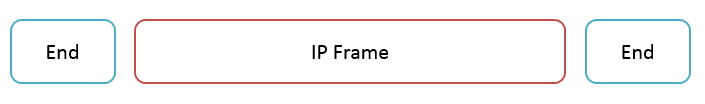
\includegraphics[scale=0.5]{ip2.png}
  \end{center}
\end{frame}

\begin{frame}{}
    \begin{block}{Vorteile}
      \begin{itemize}
        \item Sehr einfache Implementierung
        \item Sehr wenig Overhead
      \end{itemize}
    \end{block}

    \begin{alertblock}{Nachteile}
      \begin{itemize}
        \item Steuersignale können Verbindung unterbrechen (z.B. Strg-C)
        \item Keine Fehlererkennung
        \item Übertragungsrate (1,2 kbps - 19,2 kbps)
        \item Keine Meta-Daten übertragbar
      \end{itemize}
    \end{alertblock}

\end{frame}

\begin{frame}{Erweiterungs - Wünsche}
  \begin{itemize}
    \item Fehlerkorrektur
    \item Daten-Komprimierung
    \item Rechner-Adressierung
    \item Multi-Protokoll Fähigkeit
  \end{itemize}

\end{frame}

\begin{frame}{Ablösung durch PPP}
Was ist PPP?\newline
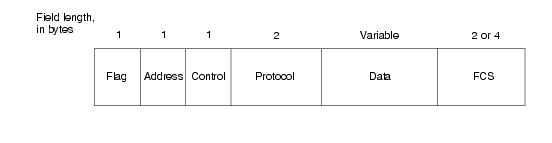
\includegraphics[scale=0.5]{ppp.jpg}
(Hübscheres Bild...)\newline
Vorteie gegenüber SLIP:\newline
(Aufzählungszeichen meiden...vlt Visualisierung)
\end{frame}

\begin{frame}{Fragen}
\begin{center}
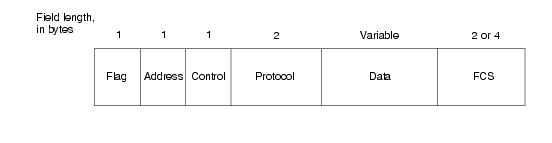
\includegraphics[scale=0.8]{ppp.jpg}
\end{center}

\end{frame}

\end{document}
